\documentclass[10pt, twocolumn]{article} 
\usepackage{simpleConference}
\usepackage{times}
\usepackage{graphicx}
\usepackage{amssymb}
\usepackage{url,hyperref}
\usepackage{mathtools}
\usepackage{algorithm}
\usepackage[noend]{algpseudocode}
\graphicspath{{./figures/}}


\begin{document}

\title{Advanced Real-time Reconstruction Methods}

\author{Conner Brooks\\
\\
CAP 4453\\
\today \\
\\
University of Central Florida\\
Orlando, FL, USA\\
\\
connerbrooks@gmail.com\\
}

\maketitle
\thispagestyle{empty}


\begin{abstract}
The paper Real Time Dense RGB-D SLAM with Volumentric Fusion \cite{whelan14} presents a new SLAM--Simultaneous Localization and Mapping--system capable of producing high quality
reconstructions of a 3 dimensional environment with a low cost RGB-D sensor e.g. the Microsoft Kinect. This system is made possible by three key techniques.
First, General-Purpose computing on Graphics Processing Units (GPGPU) and a 3D 
  cyclical buffer trick to extend the scanning volume to and unbounded spatial
  region. Second, this system also overcomes pose estimation limitations by combining
  dense geometric and photometric camera pose constraints. Third, the map of the 
  environment is updated according to place recognition and loop closure constraints.
  In this paper the initial implementation of KinectFusion \cite{izadi11} \cite{newcombe11} will be described, as well as the first 2 contributions from the paper by Whelan et al.
  
\end{abstract}



\section{Introduction}
3D reconstruction of environments is an important problem for robotics, virtual reality, and augmented reality. Understanding the geometry allows a robot to avoid obticals and navigate, and with augmented reality allows for interesting interactions with the environment. The advent of commodity depth sensors has resulted in a large amount of research concerning 3D understanding of environments. The work by Whelan et al. is the culmination of much of that work and represents one of the most advanced 3D scanning systems. To understand the work presented in this paper, one must first understand the work in the seminal paper by Newcombe et al. \cite{newcombe11}.
The purpose of these systems and their development are to provide a dense 3D mesh of the physical environment some agent--a robot or human--may be positioned in. These systems allow for full 6 degrees of freedom (6DOF) tracking of where in the environment the agent is and where it is looking--that is the agent's translation $(x, y, z)$ cartesian coordinates in space (with respect to some origin, normally where the scan begins) and rotation or where the agent is pointed. 
This is similar to previous SLAM systems, however the difference is that the map created by this system is a dense mesh which is useful especially in augmented reality applications where we want to know where a surface is in order to place a virtual object or display an interface with respect to the environment. 
The difficulty with these application is normally the tracking as it is slow and not robust enough for a common user to make efficient use of the system; KinectFusion and the extensions presented by Whelan et. al. provide a system that improves tracking to a robust enough level that a common user can scan and move through the environment. This technology has been leveraged in the new Microsoft HoloLens \cite{hololens} which is a new head mounted augmented reality system that uses many of the concepts that will be explained in this paper. 
The open-source community has made some contributions with respect to this field, providing a few different implementations of the initial KinectFusion algorithm as well as some of the extensions presented in this paper. A general overview of these implementations will be provided in section \ref{sec:opensource}. These implementations provide a good starting point for someone who may want to implement some of the extensions described in this paper. Unfortunately the source code for the implementation in the paper by Whelan et. al. was not provided.


\section{KinectFusion Overview}

\subsection{Understanding Depth Sensors}
This system takes as input multiple 2D depth images--also known as depth maps--and fuses them into a mesh. These depth maps are like normal 2D images but rather than each pixel storing a red, green, and blue value they store a single depth value, this depth image can be thought of as a 2D array or matrix of depth values. An example of this is shown in figure \ref{fig:depthimage}. 

\begin{figure}[h!]
  \centering
  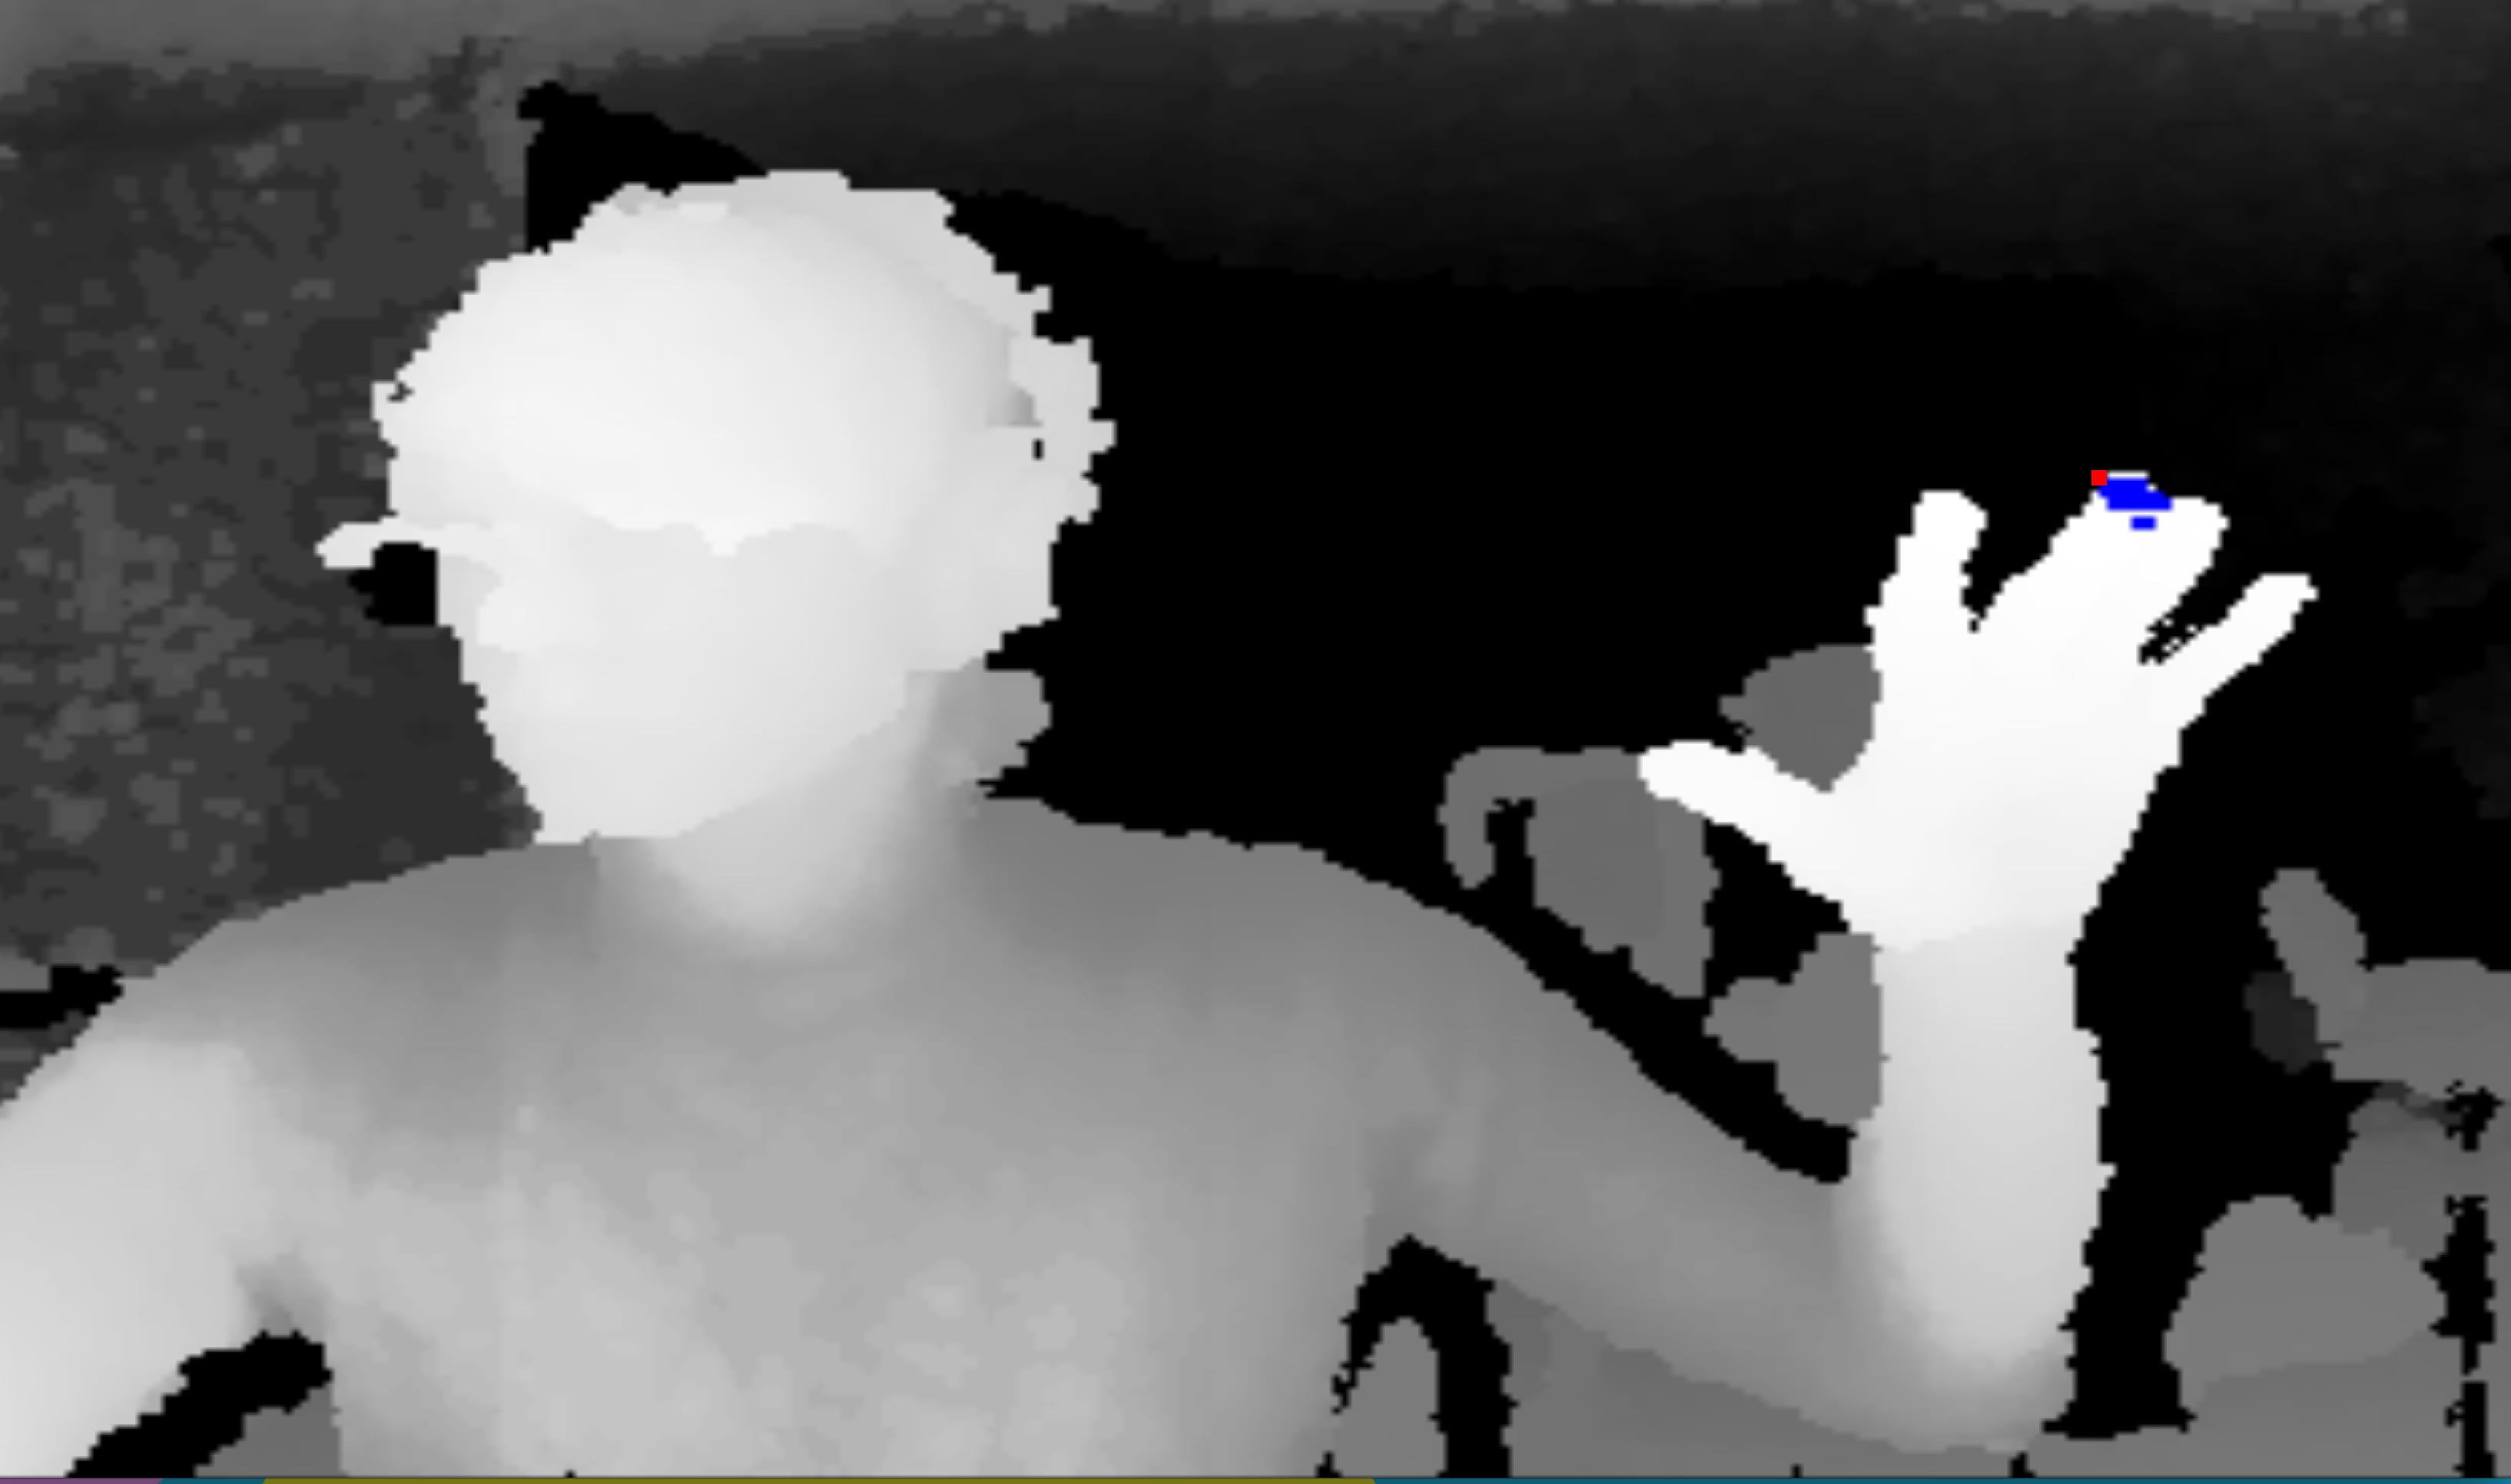
\includegraphics[width=0.8\linewidth]{depthimage}
  \caption{Depth image produced by a Depth Sensor.}
  \label{fig:depthimage}
\end{figure}

The Kinect version 1 uses a PrimeSense sensor which uses structured-light to interpret depth, this works by projecting infrared points (IR) at the scene and using an IR camera to interpret those points. The projected IR points have a calibrated pattern which is picked up by the IR camera which is shown in figure \ref{fig:ir}. All processing to determine depth from this IR image is done on the device. 

\begin{figure}[h!]
  \centering
  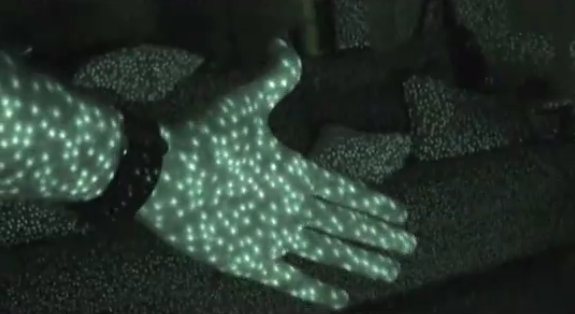
\includegraphics[width=0.8\linewidth]{KinectIR}
  \caption{Infrared light projected by the Kinect Sensor}
  \label{fig:ir}
\end{figure}


\subsection{Surface Measurement}
What we do in this step is that we take our depth image as described above and create a vertex map; this vertex map can be thought of as a point cloud or a collections of points as tuples $(x, y, z)$ in space, an example of this is shown in figure \ref{fig:pointcloud}. We also want to calculate the normal vectors for each of our given points as these normals help speed up some of the calculations we will wish to do later.

\begin{figure}
  \centering
  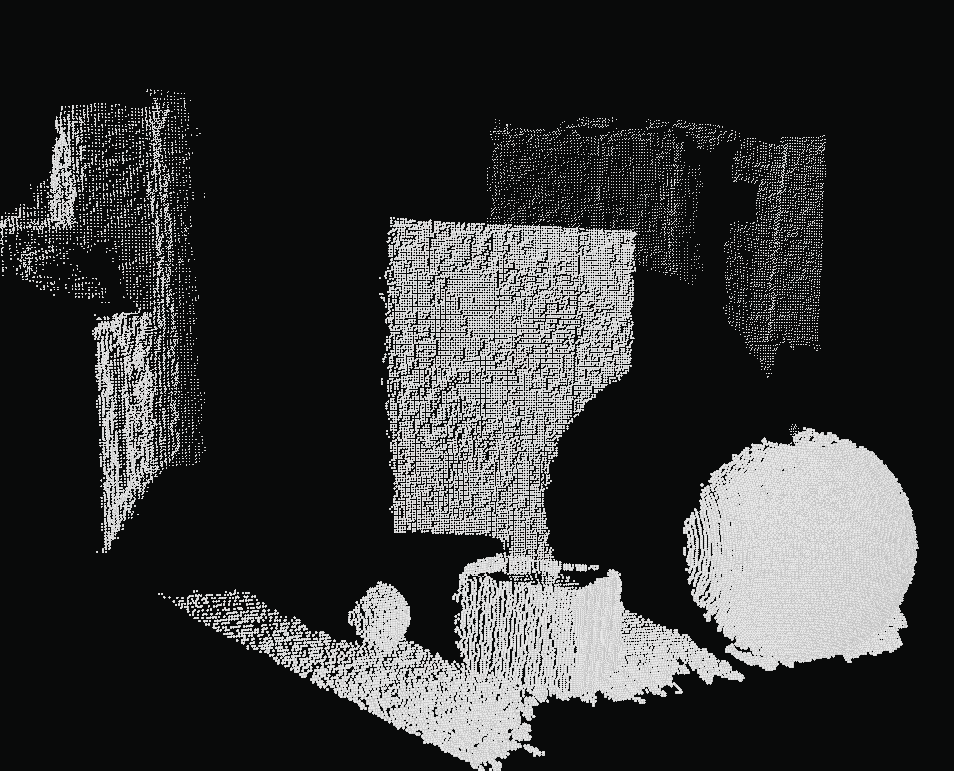
\includegraphics[width=0.8\linewidth]{pointcloud}
  \caption{Point cloud from a Kinect sensor.}
  \label{fig:pointcloud}
\end{figure}



At time $k$ raw depth map $R_k$--from the sensor--provides calibrated depth measurement $R_k(\mathbf{u}) \in \mathbb{R}$ at each image pixel $\mathbf{u} = (u,v)^{\top}$
A bilateral filter is applied $D_k(\mathbf{u})$ which will reduce noise in our depth image.
Filtered depth values are back projected into sensor frame of reference to obtain vertex map $\mathbf{V}_k$ where 

\begin{equation}
\mathbf{V}_k(\mathbf{u}) = D_k(\mathbf{u})\mathbf{K}^{-1}\dot{\mathbf{u}}
\end{equation}

where $\mathbf{K}$ is the constant calibration matrix and transforms points $\rightarrow$ image pixels, and the dot denotes homogeneous vectors $\mathbf{\dot{u}} := (\mathbf{u}^{\top}|1)^{\top}$
Since each frame is a measurment on a grid we can compute normal vectors with a cross product between neighboring map vertecies,

\begin{equation}
\mathbf{N}_k(\mathrm{u}) = v[(\mathbf{V}_k(u+1,v) - \mathbf{V}_k(u, v)) \times (\mathbf{V}_k(u,v+1) - \mathbf{V}_k(u,v))]
\end{equation}

 where $v[\mathbf{x}] = \mathbf{x} / \| \mathbf{x} \|_{2}$

We compute an $L = 3$ vertex and normal map pyramid is computed, the first level of the pyramid is the input depth map, we then down-sample this depth map to get the second level then once again to get the third level. 
Depth pyramid $D^{l \in[1\dots L]}$ bottom is original bilateral filtered depth map. 
At each level $\textbf{V}^{l \in[1\dots L]}$ $\textbf{N}^{l \in[1\dots L]}$ with the equations from the previous slide.
Given the camera $\rightarrow$ global co-ordinate frame transform $\mathsf{T}_{g,k}$, the global frame vertex is $\textbf{V}^{g}_{k} = \mathsf{T}_{g,k} \dot{\textbf{V}}_{k}(\mathrm{u})$
The equivalent mapping of normal vectors $\mathbf{N}^{g}_{k}(\mathbf{u}) = \mathsf{R}_{g,k}\mathbf{N}(\mathbf{u})$
This puts our vertex and normal maps into the global coordinate frame which is with respect to some $(0, 0, 0)$ (normally the location in which the scan was initiated).

\subsection{Mapping as Surface Reconstruction}
Each depth frame with its estimated pose, is fused into a single 3D reconstruction using a volumentric truncated signed distance function. You can think of this volume as a 3D grid that holds different values at each index. 
This TSDF will be used to generate our mesh, we will also use the TSDF as a global reference for our new scans so that we can calculate the change in pose. 
A signed distance functions value corresponds to the closest zero crossing (surface interface), taking positive values from surface $\rightarrow$ free space, and negative values on the non-visible side. Figure \ref{fig:tsdfslice} shows how the TSDF can represent surfaces as zero crossings.
The TSDF is denoted by $\mathbf{S}_{k}(\mathbf{p})$ where $\mathbf{p} \in \mathbb{R}^{3}$ is a global frame point in the TSDF with a specified resolution. The continous TSDF will be denoted by $\mathbf{S}$

\begin{figure}
  \centering
  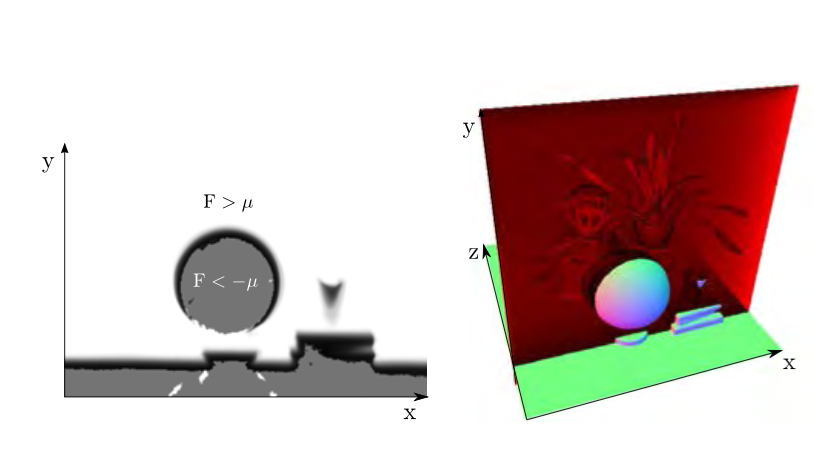
\includegraphics[width=0.8\linewidth]{tsdf}
  \caption{A slice of the truncated signed distance volume.}
  \label{fig:tsdfslice}
\end{figure}

Two Components are stored at each location of the TSDF: the current truncated signed distance value $\mathrm{F}_{k}(\mathbf{p})$ and a weight $\mathrm{W}_k(\mathbf{p})$.

\begin{equation}
\mathbf{S}_{k} \rightarrow [\mathrm{F}_{k}(\mathbf{p}), \mathrm{W}_{k}(\mathbf{p})]
\end{equation}

The TSDF is updated at an index $\mathbf{p}$ with,

\begin{equation}
\mathrm{F}_k(\mathbf{p}) = \frac{\mathrm{W}_{k-1}(\mathbf{p}) \mathrm{F}_{k-1}(\mathbf{p}) + \mathrm{W}_{\mathbf{R}_k}(\mathbf{p}) \mathrm{F}_{\mathbf{R}_k}(\mathbf{p})}{\mathrm{W}_{k-1}(\mathbf{p}) + \mathrm{W}_{\mathbf{R}_k}(\mathbf{p})}
\end{equation}

\begin{equation}
\mathrm{W}_k (\mathbf{p}) \leftarrow \mathrm{min} (\mathrm{W}_{k-1} (\mathbf{p}) + \mathrm{W} (\mathbf{p}), \mathrm{W}_{\eta})
\end{equation}

this updates the TSDFs distance value $\mathrm{F}_k$ and weight value $\mathrm{W}_k$ at the point $\mathbf{p}$ which updates our global model of the environments depth values and weight values. The weight $\mathrm{W}_k$ provides weighting of the TSDF proportional to the uncertainty of the surface measurement. It has been found that setting $\mathrm{W}_{\mathrm{R}_k} (\mathbf{p}) = 1$ resulting in a simple average, provides good results. 

\subsection{Surface Prediction from Ray Casting the TSDF}
To estimate the change in pose, we must first create a vertex and normal map from the global TSDF by casting rays into the TSDF and finding zero crossings. This pointcloude that we predict is used to calculated the rigid body transform between the current camera pose and the global model.
We can compute a dense surface prediction by rendering the surface in a virtual camera with the current estimate $\mathsf{T}_{g,k}$. 
The surface prediction is stored as a vertex and normal map $\hat{\mathbf{V}}_{k}$ and $\hat{\mathbf{N}}_{k}$ and frame of reference $k$.
This is used in the subsequent camera pose estimation step.
In the global SDF, a per pixel raycast can be performed. Each ray $\mathsf{T}_{g,k}\mathbf{K}^{-1}\mathbf{\dot{u}}$ is marched starting from min depth for pixel and stopping at a zero crossing.
For points on or close to surface interface $F_{k}(\mathbf{p}) = 0$ we assume the gradient of the TSDF at $\mathbf{p}$ is orthogonal to the zero level set, so the surface normal for the associated pixel $\mathbf{u}$ can be computed directly from $F_{k}$ using a numerical derivative of the SDF:

\begin{equation}
\mathsf{R}_{g,k} \mathbf{\hat{N}}_{k} (\mathbf{u}) = \mathbf{\hat{N}}^{g}_{k} = v[\nabla F(\mathbf{p})], \nabla F = 
\begin{bmatrix}
    \frac{\delta F}{\delta x}, & \frac{\delta F}{\delta y}, & \frac{\delta F}{\delta z}
\end{bmatrix}^{\top}
\end{equation}

This provides us with an approximated vertex and normal map which is used in the sensor pose estimation step as the comparison previous vertex and normal map.


\subsection{Sensor Pose Estimation}
Now that we have our vertex and normal map from our current frame and the global model we can estimated the change in pose for this frame. This will allow our new frame to be fused into the TSDF at the correct location.

The live 6DOF camera pose estimated for a frame at time k that is the rotation $\mathsf{R}_{g,k}$ and translation $\mathbf{t}_{g,k}$

\begin{equation}
\mathsf{T}_{g,k} = 
\begin{bmatrix}
  \mathsf{R}_{g,k} & \mathbf{t}_{g,k} \\
  0 & 1
\end{bmatrix}
\in \mathbb{SE}_{3}
\end{equation}

where $\mathbb{SE}_{3} := \{\mathsf{R}, \mathbf{t}\ |\ \mathsf{R} \in \mathbb{SO}_{3}, \mathbf{t} \in \mathbb{R}^{3}\}$

\hfill \break

To track the sensor frame, the live surface measurement $(\mathbf{V}_{k}, \mathbf{N}_{k})$ against the model prediction from the previous frame $(\mathbf{\hat{V}}_{k-1}, \mathbf{\hat{N}}_{k-1})$. First we must find correspondences between the two sets of points with projective data association. 


\begin{algorithm}
\caption{Projective point-plane data association.}\label{euclid}
\begin{algorithmic}[1]
\For{each image pixel $u \in$ depth map $\mathbf{D}_i$ \textbf{in parallel}}
\If {$\mathbf{D}_i(u) > 0$} 
\State $\mathbf{v}_{i-1} \leftarrow \mathbf{T}^{-1}_{i-1} \mathbf{v}^{g}_{i-1}$
\State $\mathbf{p} \leftarrow$ perspective project vertex $\mathbf{v}_{i-1}$
\If {$\mathbf{p} \in$ vertex map $\mathbf{V}_i$}
\State $\mathbf{v} \leftarrow \mathbf{T}_i \mathbf{V}_i(p)$
\State $\mathbf{n} \leftarrow \mathbf{R}_i \mathbf{N}_i(p)$
\If {$\|\mathbf{v} - \mathbf{v}^{g}_{i-1} \| <$ distance threshold and $abs(\mathbf{n} \cdot \mathbf{n}^{g}_{i-1}) <$ normal threshold}
\State point correspondence found
\EndIf
\EndIf
\EndIf
\EndFor
\end{algorithmic}
\end{algorithm}


Given these correspondences the output of each ICP iteration is a single transformation matrix $T$ which minimizes the point to plane error metric, or the sum of squared distances between each point in the current frame and the tangent plane at corresponding points in the previous frame. Figure \ref{fig:pointplane} \cite{Low04linearleast-squares} provides a visual explanation of how this point to plane error metric works in 2D.

\begin{equation}
\mathbf{E}(\mathsf{T}_{g,k}) = 
\sum_{\substack{
   \mathbf{u} \in \mathcal{U} \\
   \Omega_{k}(\mathbf{u}) \neq null
  }}
  \| ( \mathsf{T}_{g,k} \mathbf{\dot{V}} (\mathbf{u}) - \mathbf{\hat{V}}^{g}_{k-1} (\mathbf{\hat{u}}))^{\top} \mathbf{\hat{N}}^{g}_{k-1} (\mathbf{\hat{u}}) \|_{2}
\end{equation}


A linear approximation is used to solve this system, we assume that the transformation between two frames is incremental.

\begin{figure}
  \centering
  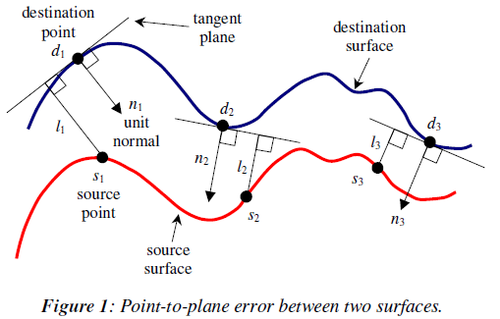
\includegraphics[width=1.0\linewidth]{pointplane}
  \caption{Point-to-plane error between two surfaces.}
  \label{fig:pointplane}
\end{figure}

\subsection{Bringing it All Together}
Now that we have seen how each system works separately it helps to see how each piece works together to make this system work as well as it does. Figure \ref{fig:workflow} shows how each output from each calculation we have made is used in the system. To summarize, the input image $\mathsf{R}_k$ is passed to the surface measurement component and the component that updates our current reconstruction. From the measurement we pass our surface vertex and normal maps $\mathbf{V}_k$ and $\mathbf{N}_k$ to the pose estimation component, this also requires our predicted vertex and normal maps as well as the global pose as we must calculate the transform with respect to our model. The pose we calculated is sent to the reconstruction updating component where the frame $\mathsf{R}_k$ is integrated into our Global TSDF, in the prediction phase we raycast our current TSDF to come up with our predicted vertex and normal maps. This process is fast enough for this system to run at 30 frames per second. Figure \ref{fig:visworkflow} shows a more visual overview of the system.

\begin{figure}
  \centering
  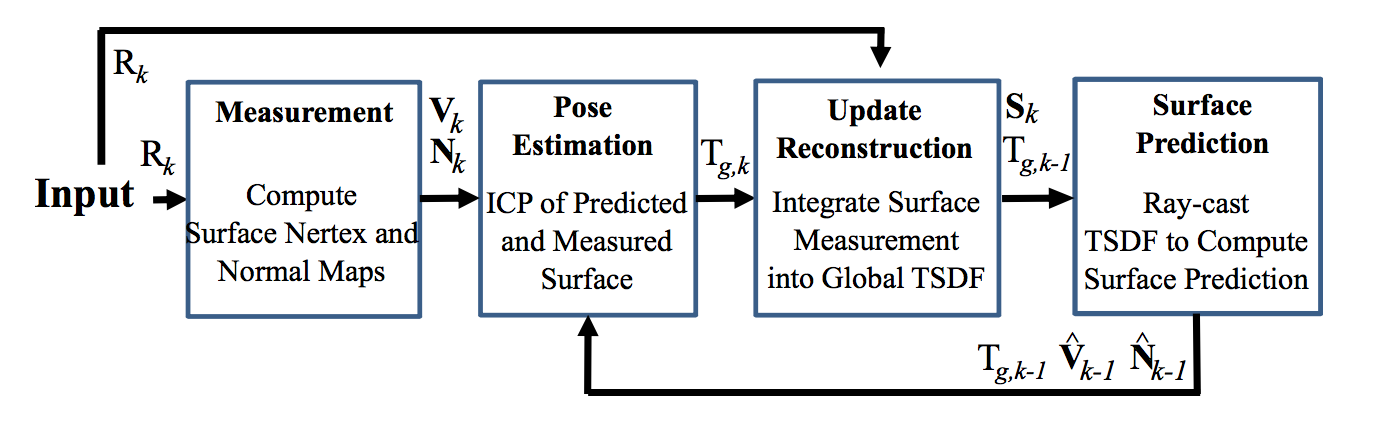
\includegraphics[width=1.0\linewidth]{workflow}
  \caption{Overview of the KinectFusion system.}
  \label{fig:workflow}
\end{figure}

\begin{figure}
  \centering
  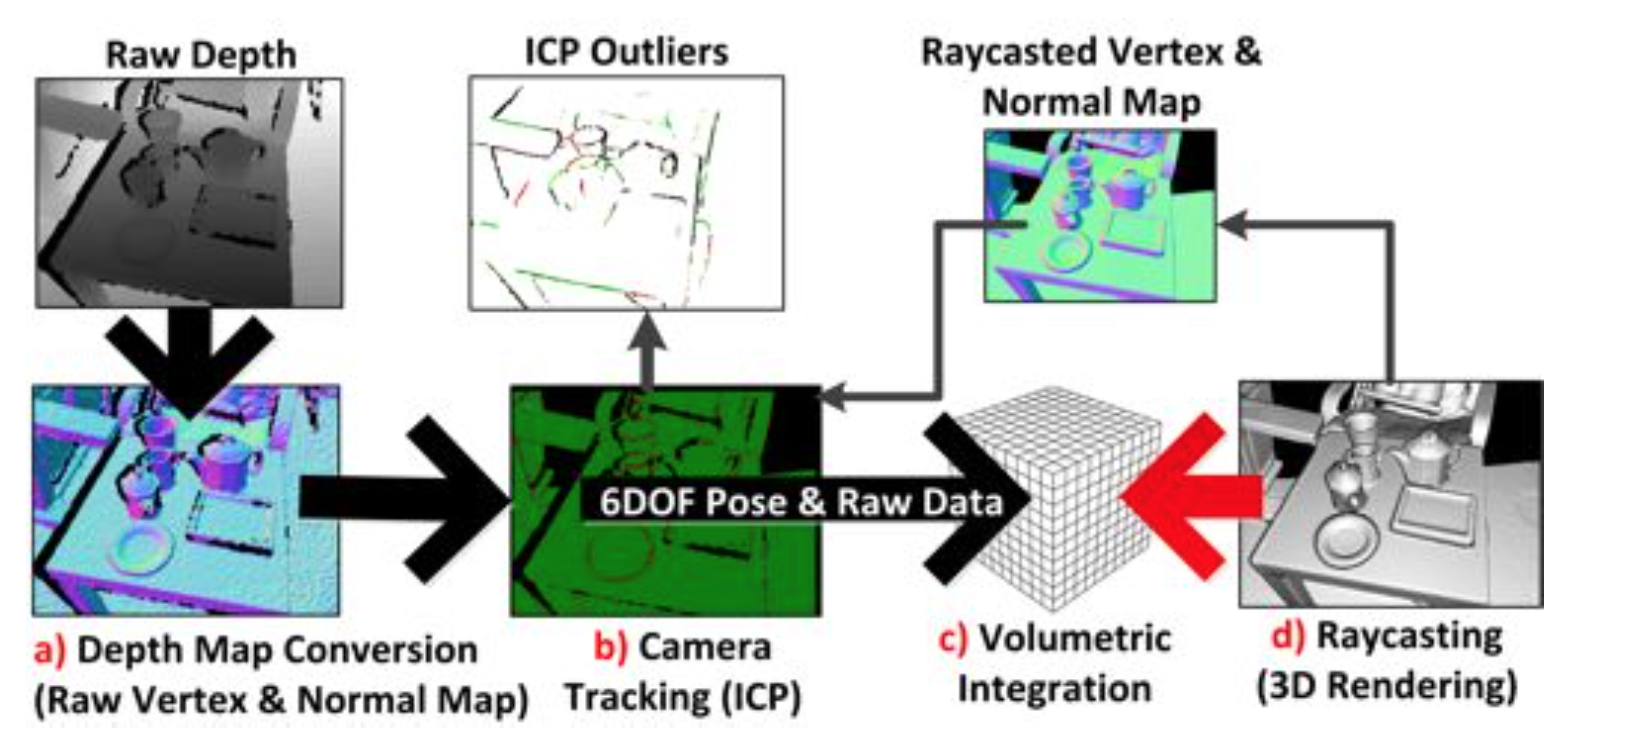
\includegraphics[width=1.0\linewidth]{kinectfusion}
  \caption{Overview of the KinectFusion system.}
  \label{fig:visworkflow}
\end{figure}



\section{Extensions to Kinect Fusion}
Now we move to the extension of this algorithm presented by Whelan et. al \cite{whelan14}. This section will cover the cyclical buffer trick used which allows unlimited volumes to be scanned as well as improved camera estimates using photometric pose estimation which improves overall model accuracy.

\subsection{Cyclical Buffer Trick}
The first contribution of this paper is a cyclical buffer trick that allows the maximum volume that we can scan to be infinitely large. In the initial KinectFusion implementation the volume was limited by how large GPU memory was as the TSDF must be stored in GPU memory in order for the application to run at 30 fps. This contribution allows the GPU memory to be reused and the scanned areas to be saved to computer memory extending the maximum volume.

The position of the TSDF volume in the global frame is initially $\mathbf{g}_{0} = (0, 0, 0)^{\top}$
When our pose estimate leaves a movement threshold $m_{s}$ around $\mathbf{g}_{i}$ will cause a volume shift.
The shift triggers and the TSDF is virtually translated about the camera pose (in voxel units) to bring the camera's position to $\mathbf{g}_{i+1}$.
To compute the new camera pose, we must compute the number of voxel units crossed,

\begin{equation}
u = \lfloor \frac{v_{s}t^{T}_{i+1}}{v_d} \rfloor
\end{equation}

then shift the pose, updating the global position of the TSDF,

\begin{equation}
\mathbf{t}^{T'}_{i+1} = \mathbf{t}^{T}_{i+1} - \frac{v_{d}\mathbf{u}}{v_{s}}
\end{equation}

\begin{equation}
\mathbf{g}_{i+1} = \mathbf{g}_{i} + \mathbf{u}
\end{equation}

\begin{figure}
  \centering
  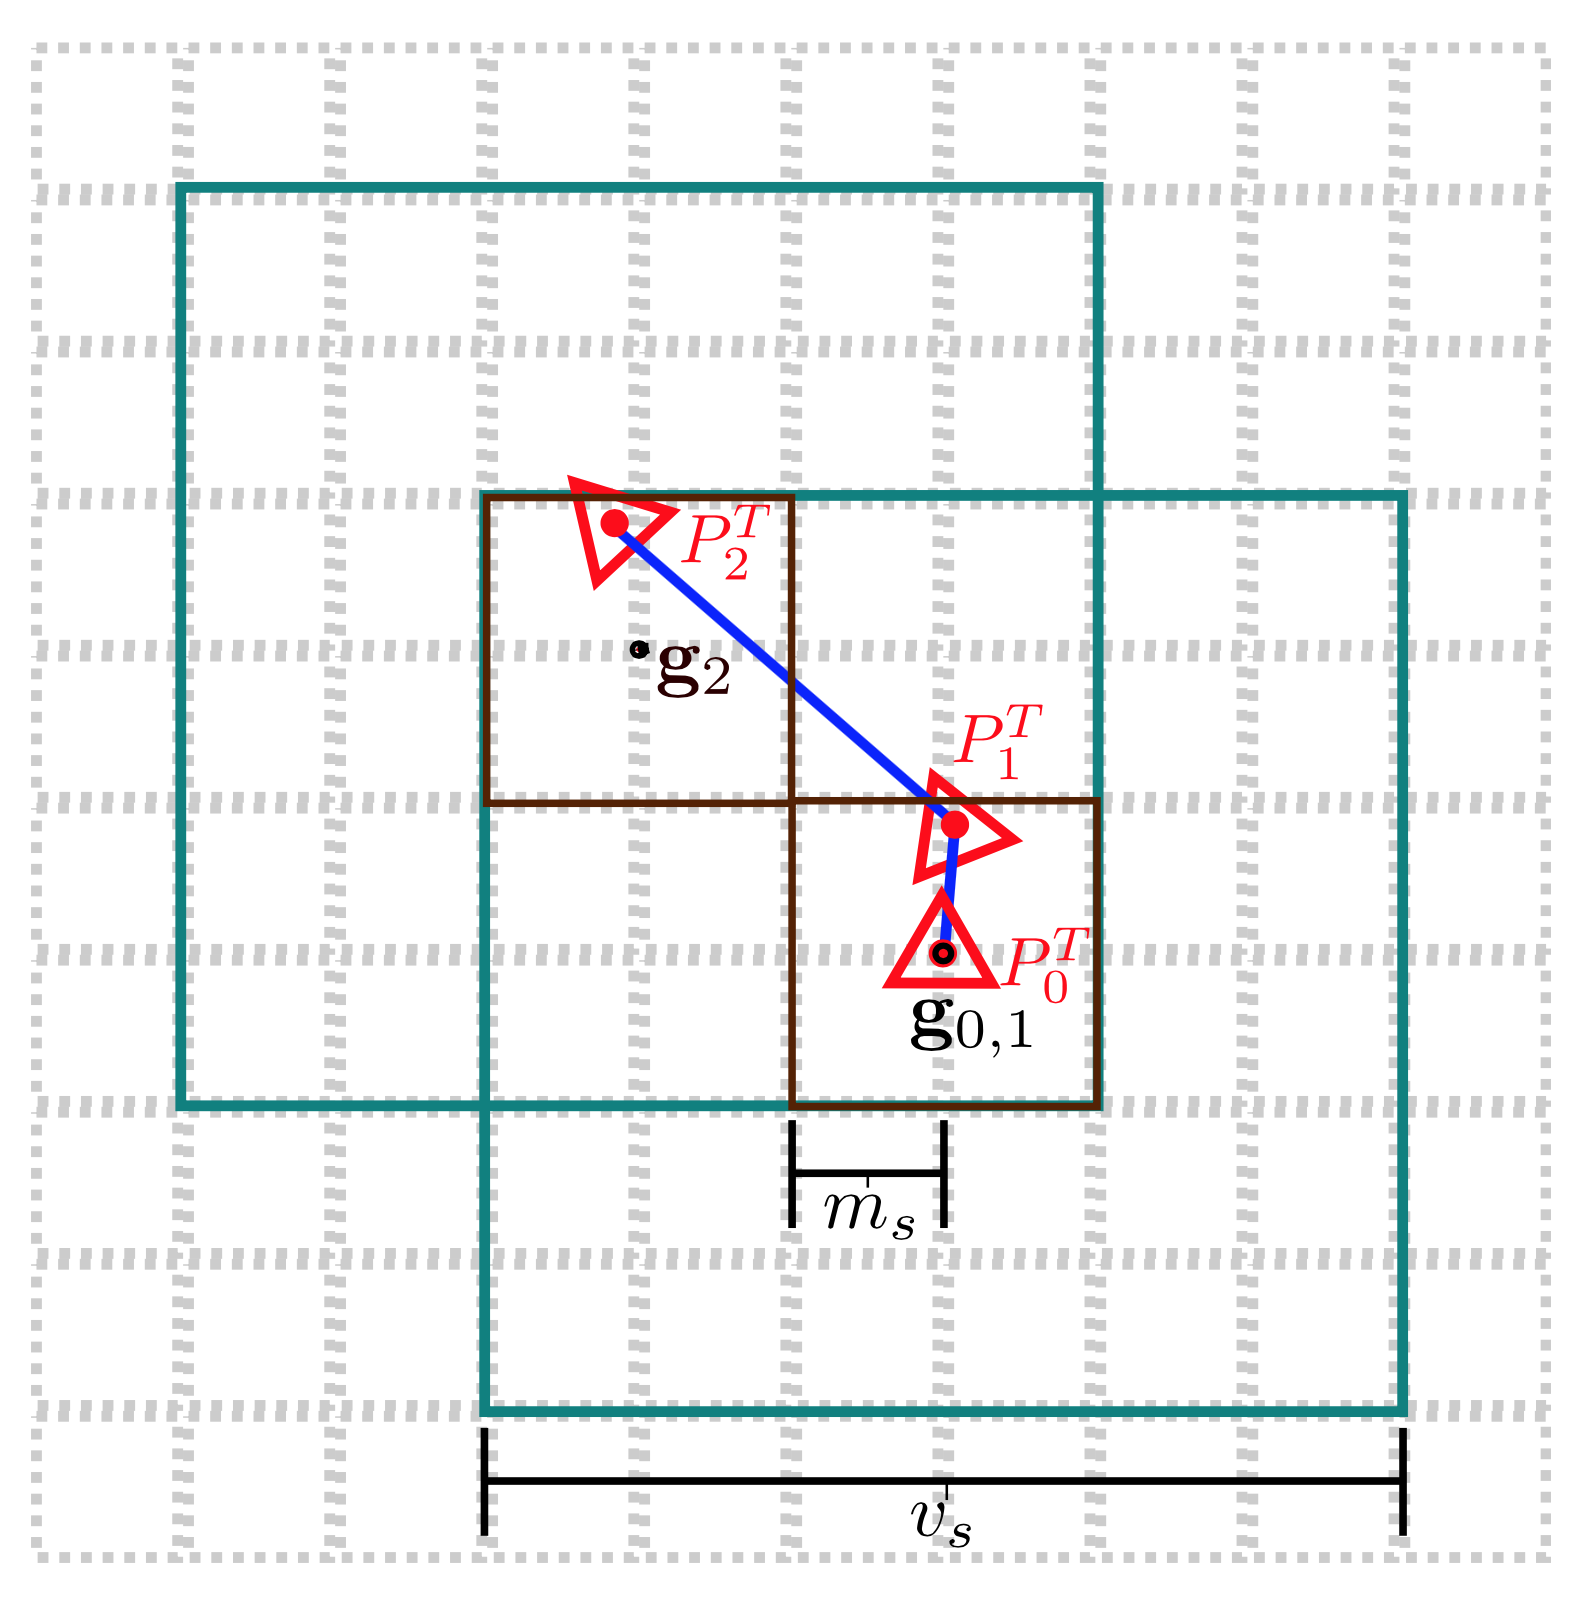
\includegraphics[width=0.8\linewidth]{tsdfshift}
  \caption{This shows the movement threshold $m_s$ and how the TSDF volume shifts when the camera moves outside of the bounds of this threshold.}
  \label{fig:tsdfshift}
\end{figure}

This process is shown in figure \ref{fig:tsdfshift}.


This creates what is referred to as a cloud slice, this cloud slice is part of the whole TSDF. This cloud slice gets passed to a greedy triangulation algorithm to create the mesh, and is then stored in computer memory. This allows the volume we wish to scan to be as large as we wish, as the mesh stored in memory will be paged to disk. A visualization of this process is shown in figure \ref{fig:cloudslice}.

\begin{figure}
  \centering
  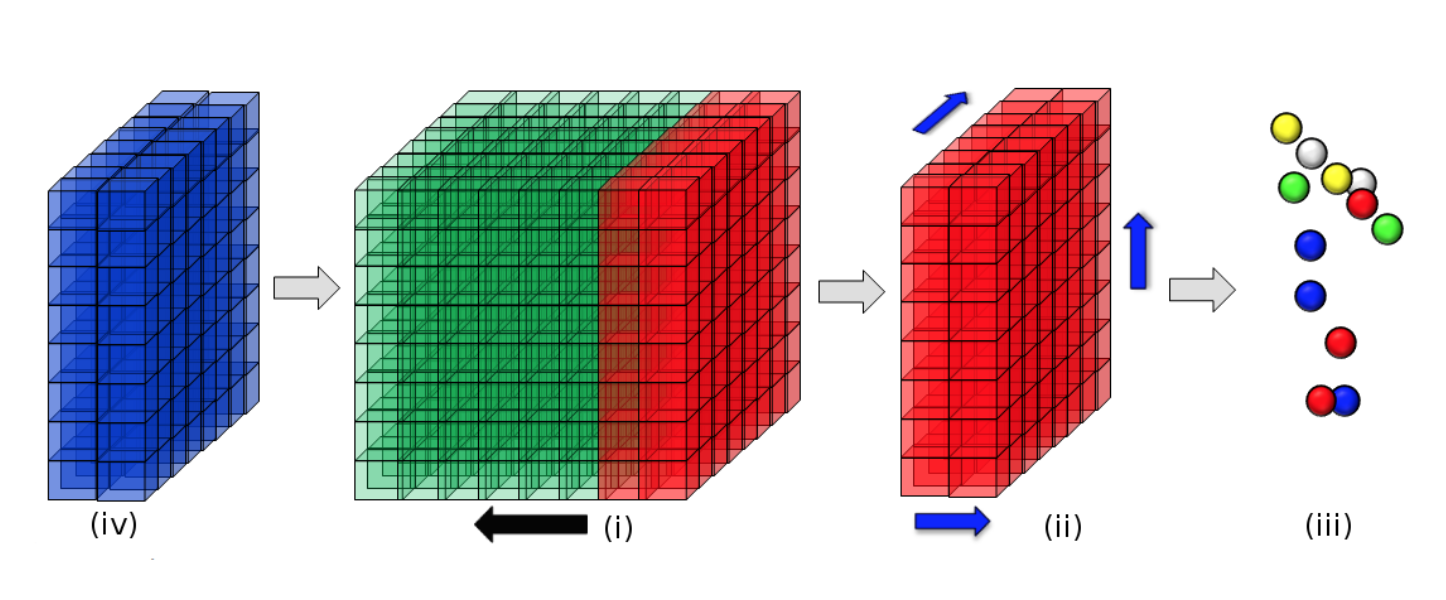
\includegraphics[width=1.0\linewidth]{cloudslice}
  \caption{Visualization of the volume shifting process, (i) The camera motion exceeds the movement threshold ms (direction of camera motion shown by the black arrow); (ii) Volume slice leaving the volume (red) is raycast along all three axes to extract surface points and reset to free space; (iii) The raycast surface is extracted as a point cloud and fed into the Greedy Projection Triangulation (GPT) algorithm of Marton et al. (2009); (iv) New region of space (blue) enters the volume and is integrated using new modulo addressing of the volume.}
  \label{fig:cloudslice}
\end{figure}



\subsection{Photometric Camera Pose Estimation}
The second major contribution of this paper is its combination of photometric and geometric pose estimation. Rather than relying solely on iterative closest points it adds a second estimate that uses the RGB data from the Kinect. This provides a more accurate estimate of the pose so that when we fuse a new depth image its points are more accurate with respect to the entire model.

Given two consecutive RGB-D frames $[\mathbf{rgb}_{n-1}, \mathbf{d}_{n-1}]$ and $[\mathbf{rgb}_{n}, \mathbf{d}_{n}]$
A rigid transform is computed between the two that maximizes photo-consistency. 
We define $V: \Omega \rightarrow \mathbb{R}^{3}$ to be back-projection of point $\mathbf{p}$ dependent on
a metric depth map $M: \Omega \rightarrow \mathbb{R}$ and
a camera intrinsics matrix $\mathbf{K} \rightarrow$ principle points $c_{x}, c_{y}$ and focal lengths $f_{x}, f_{y}$ 

\begin{equation}
V(\mathbf{p}) = \left( \frac{(\mathbf{p}_{x} - c_{x})M(\mathbf{p})}{f_{x}}, \frac{(\mathbf{p}_{y} - c_{y})M(\mathbf{p})}{f_{y}}, M(\mathbf{p}) \right)^{\top}
\end{equation}

A perspective projection of a 3D point $\mathbf{v} = (x,y,z)^{\top}$ is defined, as well as a dehomogenization by $\Pi(\mathbf{v}) = (x/z, y/z)^{\top}$. The cost to be minimised depends on the difference in intensity values between the two images $I_{n-1}, I{n}: \Omega \rightarrow \mathbb{N}$

\begin{equation}
\mathbf{E}_{rgbd} = 
\sum_{\substack{
   \mathbf{p} \in \mathcal{L} 
  }}
  \| I_{n}(\mathbf{p} - I_{n-1}(\Pi_{n-1}(exp(\xi)\mathbf{T}V_{n}(\mathbf{p})))  \|^{2}
\end{equation}

where $\mathcal{L}$ is the list of valid interest points are populated by algorithm 2 on the last page, and $\mathbf{T}$ is the current estimate of the transform. Algorithm 2 shows how the interest point correspondences are accumulated.




\subsection{Combined Camera Pose Estimation}
Now that we have two estimates of the pose we create a combined estimate by weighting the RGBD estimate against the ICP estimate. This will improve our overall estimate of pose and make the global model more accurate overall


\begin{equation}
E = E_{icp} + w_{rgbd}E_{rgbd}
\end{equation}

where $w_{rgbd}$ is the weight and was set empirically to 0.1 to refelect the difference in metrics used for ICP and RGBD costs.

For each step a linear least-squares problem  is minimized by solving:
% TODO least squares equation

\begin{equation}
\begin{bmatrix}
       \mathbf{J}_{icp} \\[0.3em]
       v \mathbf{J}_{rgbd} \\[0.3em]
\end{bmatrix}^{\top}
\begin{bmatrix}
       \mathbf{J}_{icp} \\[0.3em]
       v \mathbf{J}_{rgbd} \\[0.3em]
\end{bmatrix}
\xi
=
\begin{bmatrix}
       \mathbf{J}_{icp} \\[0.3em]
       v \mathbf{J}_{rgbd} \\[0.3em]
\end{bmatrix}^{\top}
\begin{bmatrix}
       \mathbf{r}_{icp} \\[0.3em]
       \mathbf{r}_{rgbd} \\[0.3em]
\end{bmatrix}
\end{equation}

\begin{equation}
(\mathbf{J}^{\top}_{icp} \mathbf{J}_{icp} + w_{rgbd} \mathbf{J}^{\top}_{rgbd} \mathbf{J}_{rgbd}) \xi = \mathbf{J}^{\top}_{icp} \mathbf{r}_{icp} + v \mathbf{J}^{\top}_{rgbd} \mathbf{r}_{rgbd}
\end{equation}

where $v = \sqrt{w_{rgbd}}$. The products $\mathbf{J}^{\top}\mathbf{J}$ and $\mathbf{J}^{\top} \mathbf{r}$ are computed on the GPU using a tree reduction. The final estimate returns a locally optimal camera pose which minimizes the photometric error between the RGB-D frame and the last and the geometric error between the current depth frame and the TSDF surface reconstruction.


\section{Open Source Implementations} \label{sec:opensource}
There are a few open source implementations of the KinectFusion system and its extensions. 
\begin{enumerate}
  \item Microsoft KinectFusion \cite{MSKinectFusion}
  \item KFusion \cite{kfusion}
  \item KinFu from Point Cloud Library (PCL) \cite{kinfu}
  \item RXKinFu a fork of PCL KinFu from Northeastern University \cite{RXKinFu}
\end{enumerate}

I have built an run each of these implementations except RXKinFu.  Many of these implementations have issues with tracking, there is generally no recovery so if you get into a bad state you will have to restart your scan. Many of them leave much to be desired, I began working on adding my extensions to these systems by extending KinFu Large Scale.

\subsection{Microsoft KinectFusion}
This implementation has partial code availability it comes with the new Kinect SDK, it is limited to a fixed volume. It is not fully open-source as some of the headers access closed source libraries that implement many of the important functions that comprise the system. 

\subsection{KFusion}
KFusion is an implementation of the initial KinectFusion algorithm based on the paper by Newcombe et. al. It is a standalone application with a very simple structure that is helpful to understand each individual part of the system.

\subsection{KinFu}
KinFu is a fully open source implementation from the Point Cloud Library team, there are 2 implementations available a fixed volume version KinFu and a large scale version KinFu Large Scale which uses the cyclical buffer trick presented in this paper to extend its volume. The main issue with this implementation is that it is not standalone it requires you to compile almost all of the point cloud library which, depending on your environment may take a considerable amount of time.

\subsection{RXKinFu}
This is a standalone fork of KinFu and provides the extended volume features presented in this paper. As well as some other enhancements to the overall system.




\bibliographystyle{abbrv}
\bibliography{reconstruction}


\includegraphics[width=1.0\linewidth]{algorithm2}
\includegraphics[width=1.0\linewidth]{algorithm3}

\end{document}
